\documentclass[12pt]{article}
\usepackage{amsmath,graphicx}
\pagestyle{empty}

\oddsidemargin  -0.5 cm
\evensidemargin 0.0 cm
\textwidth      6.5in
\headheight     0.0in
\topmargin      -1 cm
\textheight=9.0in

\begin{document}

\section*{Formalism for another source of interference with an arbitrary phase
relative to $q\bar{q}$}

The total amplitude is the sum of four amplitudes $A = A_c + A_{q\bar{q}} + A_{ggg}
+ A_{ggg\mbox{\scriptsize -noint}}$:
\begin{enumerate}
  \item $A_c$: continuum $q\bar{q}$,
  \item $A_{q\bar{q}}$: $\Upsilon \to q\bar{q}$,
  \item $A_{ggg}$: $\Upsilon \to ggg$ decays which interfere with
  $q\bar{q}$ at the hadron level, and
  \item $A_{ggg\mbox{\scriptsize -noint}}$: $\Upsilon \to ggg$ decays
  which do not interfere with $q\bar{q}$ at the hadron level.
\end{enumerate}
The squared amplitude is
\begin{multline}
|A|^2 = |A_c|^2 + |A_{q\bar{q}}|^2 + |A_{ggg}|^2 + |A_{ggg\mbox{\scriptsize -noint}}|^2 +
2 {\mathcal Re}({A_c}^* A_{q\bar{q}}) + 2 {\mathcal Re}({A_c}^* A_{ggg}) + \\ + 2 {\mathcal Re}({A_{q\bar{q}}}^* A_{ggg}) +
{A_{ggg\mbox{\scriptsize -noint}}}^*(A_c + A_{q\bar{q}} + A_{ggg})
\end{multline}
The only two relevant terms are $2 {\mathcal Re}({A_c}^* A_{q\bar{q}})$ and $2
{\mathcal Re}({A_c}^* A_{ggg})$.  The rest are non-interfering or are
interference between two $\Upsilon$ final states, which is just part
of the $\Upsilon$ cross-section (a part of the $\Gamma_{ee}$ we wish
to measure).

To use Karl's existing code, I need to make these two interference
terms look like one.  Karl's lineshape takes two inputs, $y_{int}$ and
$\phi$ to define interference with the background:
\begin{equation}
2{\mathcal Re}({A_c}^* A_{BW}) = y_{int} \sigma_{BW}
\left(2\frac{W_{res} - M_\Upsilon}{\Gamma} \cos\phi + \sin\phi \right)
\end{equation}
With only $q\bar{q}$ interference, $y_{int}$ is proportional to
$\sqrt{{\mathcal B}_{q\bar{q}}}$ and the amplitude of $\Upsilon \to
q\bar{q}$, and $\phi$ is the phase difference between continuum
$q\bar{q}$ and $\Upsilon \to q\bar{q}$ when $\sqrt{s} \ll M_\Upsilon$.
My $A_{BW}$ has two terms, $A_{q\bar{q}} + A_{ggg}$.  I will
parameterize them like this:
\begin{equation}
A_{q\bar{q}} = a_{q\bar{q}} e^{i\phi_r}  \mbox{ and }  A_{ggg} = a_{ggg} e^{i\phi_r + i\phi_{ggg}}
\end{equation}
where $\phi_r$ is the resonance phase (which varies from $0$ to $\pi$
as a function of beam energy) and $\phi_{ggg}$ is a constant offset due to
$\Upsilon \to q\bar{q}$ and $\Upsilon \to ggg$ not being coherent
($\phi_{ggg}$ might be $\pi$).  Now
\begin{equation}
A_{q\bar{q}} + A_{ggg} = (a_{q\bar{q}} + a_{ggg} e^{i\phi_{ggg}}) e^{i\phi_r} = (a_{q\bar{q}} + a_{ggg}
\cos\phi_{ggg} + i a_{ggg} \sin\phi_{ggg}) e^{i\phi_r} \\
\end{equation}
\begin{equation}
= \sqrt{{a_{q\bar{q}}}^2 + {a_{ggg}}^2 + 2 a_{q\bar{q}} a_{ggg} \cos\phi_{ggg}} \, \exp\left(i\phi_r +
i\tan^{-1}\left(\frac{a_{ggg} \sin\phi_{ggg}}{a_{q\bar{q}} + a_{ggg}\cos\phi_{ggg}} \right)\right)
\end{equation}
To use Karl's function, I need to replace
\begin{eqnarray}
y_{int} &\to& \sqrt{{y_{q\bar{q}}}^2 + {y_{ggg}}^2 + 2 y_{q\bar{q}}
y_{ggg} \cos\phi_{ggg}} \mbox{ and} \\
\phi &\to& \phi_{q\bar{q}} + tan^{-1} \left(\frac{y_{ggg} \sin\phi_{ggg}}{y_{q\bar{q}} + y_{ggg}\cos\phi_{ggg}} \right)
\end{eqnarray}
where $y_{q\bar{q}}$ is the usual interference parameter, $y_{ggg}$ is
the equivalent for the fraction of $\Upsilon \to ggg$ that interferes,
and $\phi_{q\bar{q}}$ is the usual starting interference (assumed to
be zero, as usual).

\pagebreak

\mbox{ }

\vfill

\includegraphics[width=\linewidth]{interference-a}

\vfill

\mbox{(The horizontal lines represent one unit in $\chi^2$)}

\pagebreak

\mbox{ }

\vfill

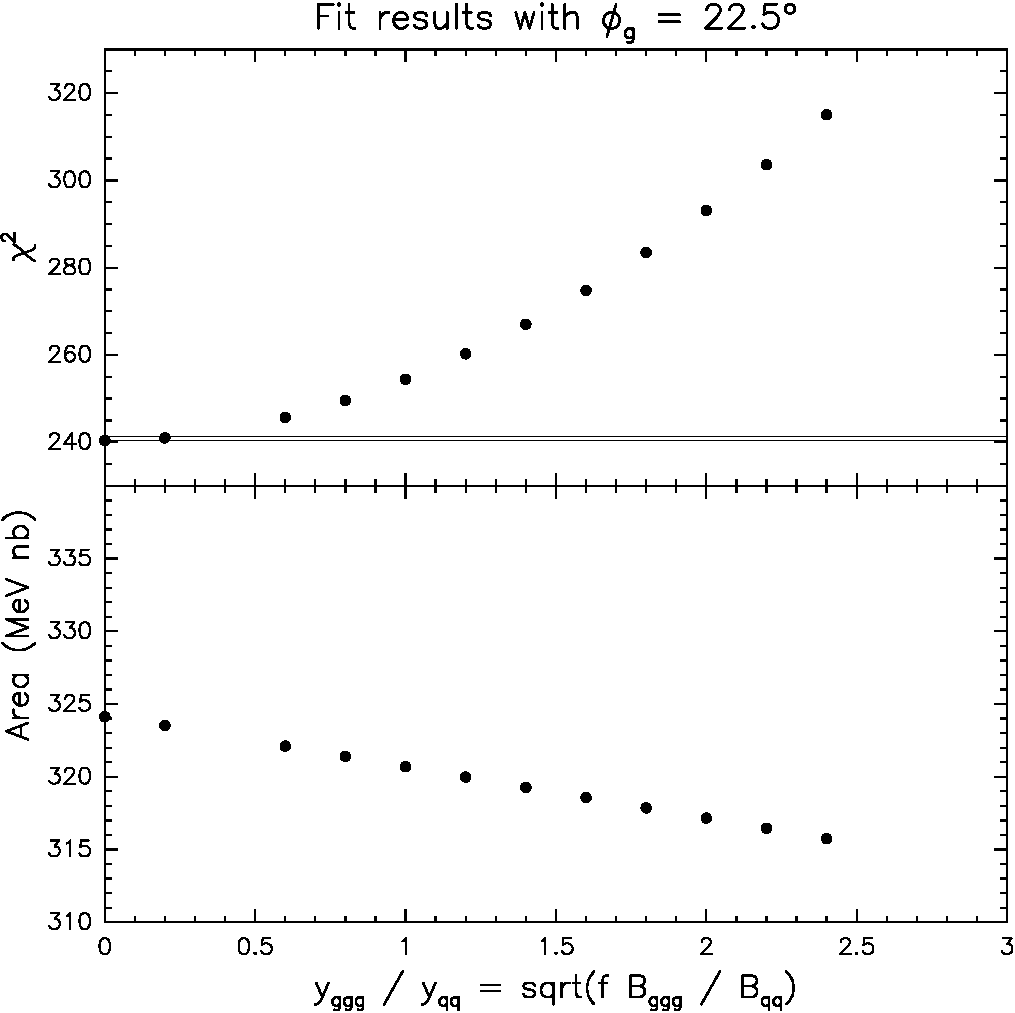
\includegraphics[width=\linewidth]{interference-b}

\vfill

\mbox{ }

\pagebreak

\mbox{ }

\vfill

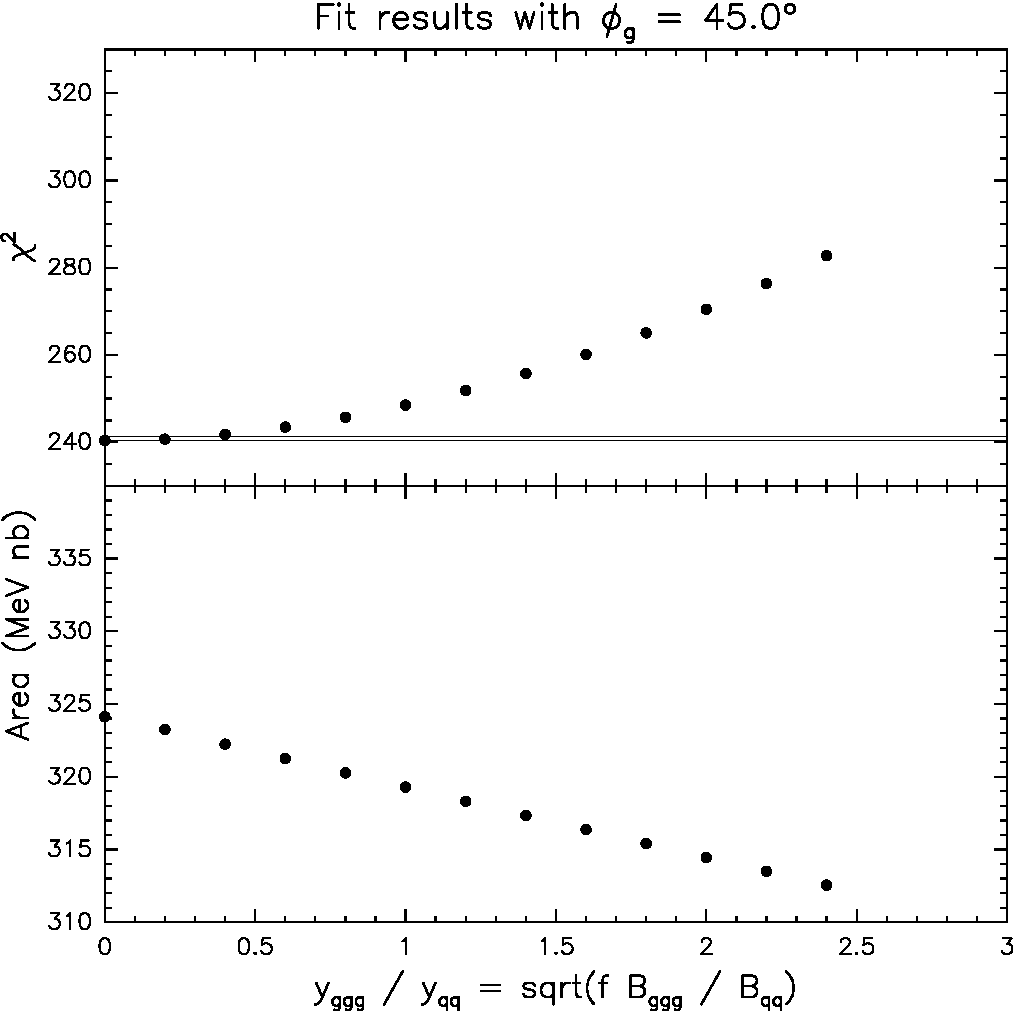
\includegraphics[width=\linewidth]{interference-c}

\vfill

\mbox{ }

\pagebreak

\mbox{ }

\vfill

\includegraphics[width=\linewidth]{interference-d}

\vfill

\mbox{ }

\pagebreak

\mbox{ }

\vfill

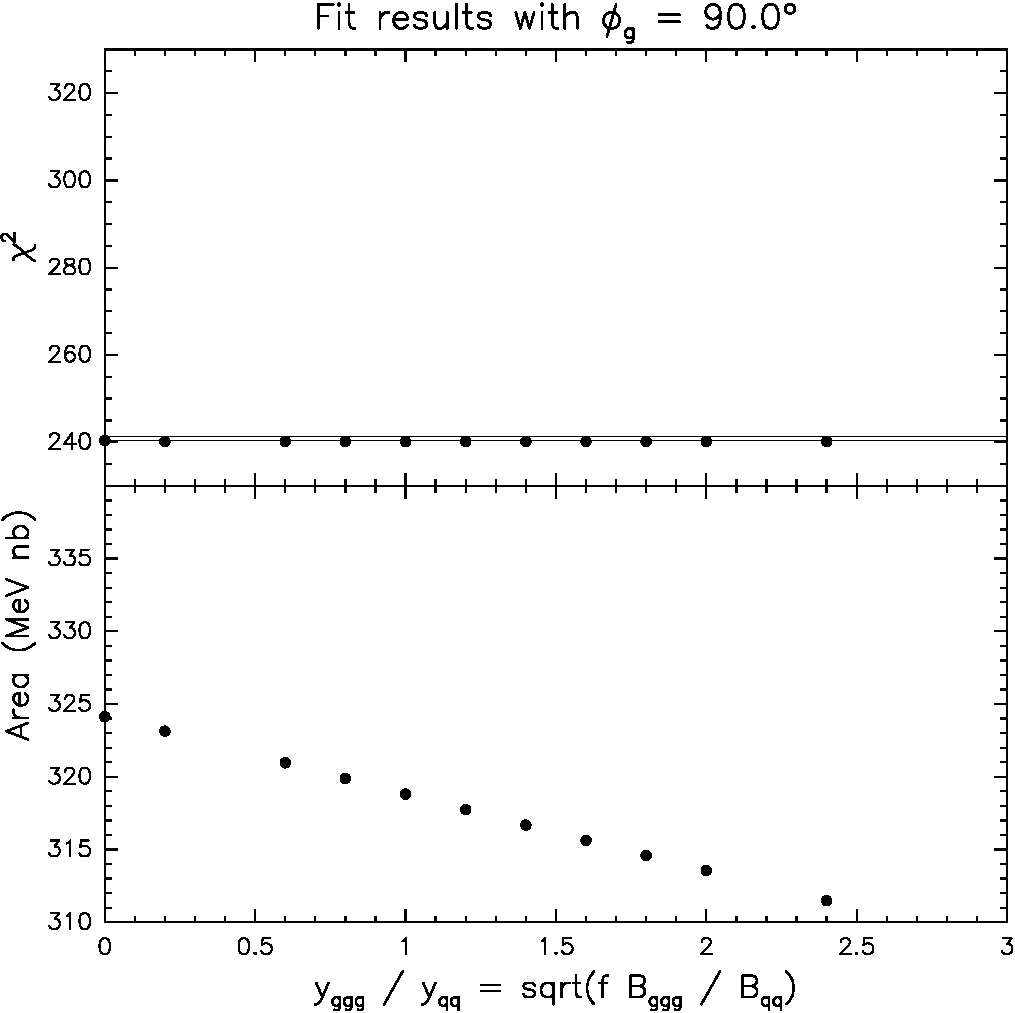
\includegraphics[width=\linewidth]{interference-e}

\vfill

\mbox{ }

\pagebreak

\mbox{ }

\vfill

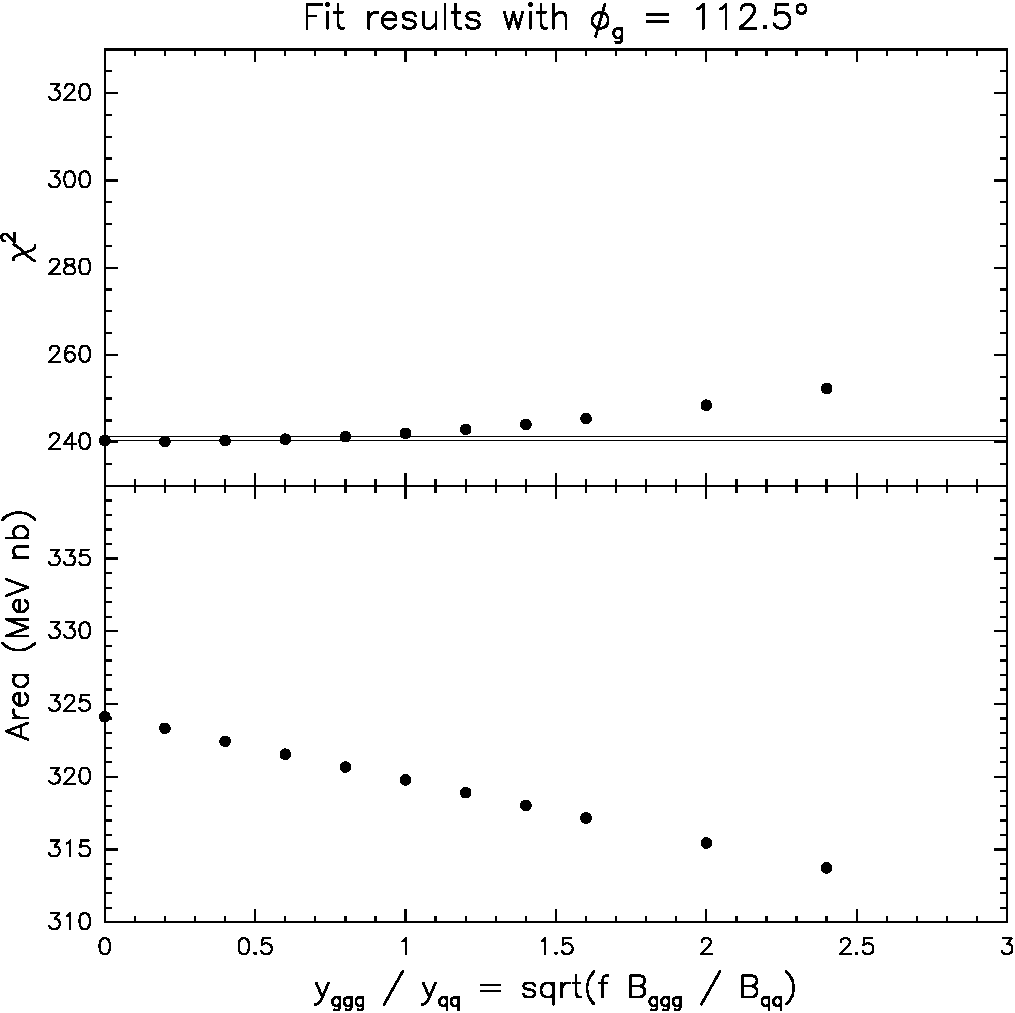
\includegraphics[width=\linewidth]{interference-f}

\vfill

\mbox{ }

\pagebreak

\mbox{ }

\vfill

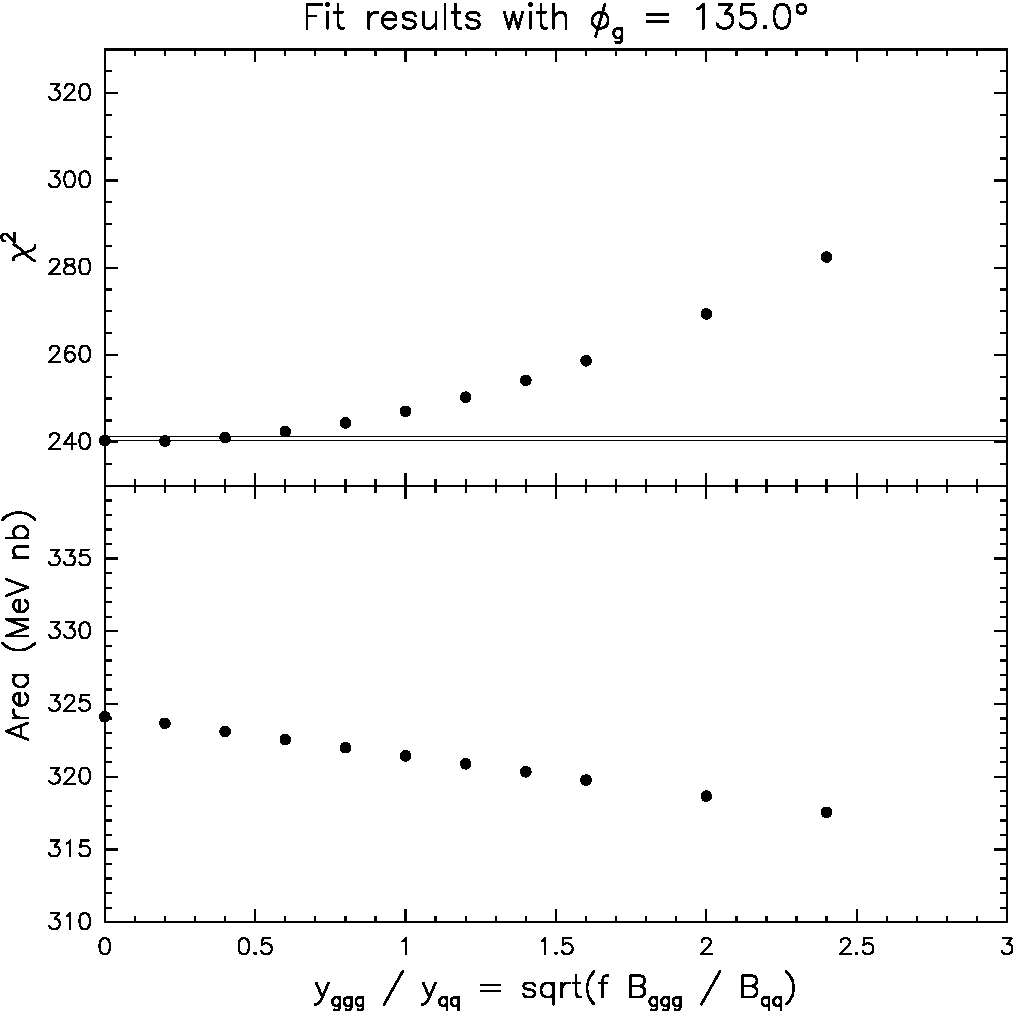
\includegraphics[width=\linewidth]{interference-g}

\vfill

\mbox{ }

\pagebreak

\mbox{ }

\vfill

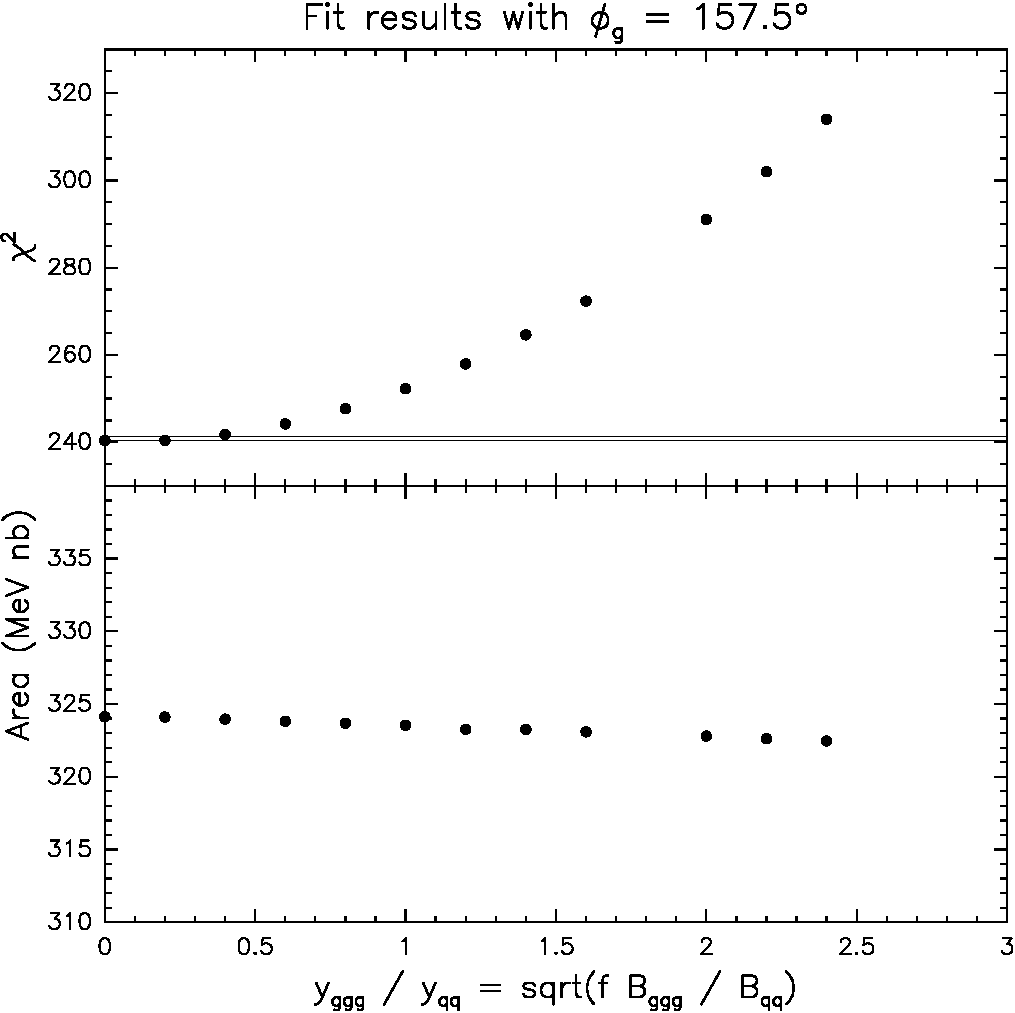
\includegraphics[width=\linewidth]{interference-h}

\vfill

\mbox{ }

\pagebreak

\mbox{ }

\vfill

\includegraphics[width=\linewidth]{interference-i}

\vfill

\mbox{ }

\pagebreak

\mbox{ }

\vfill

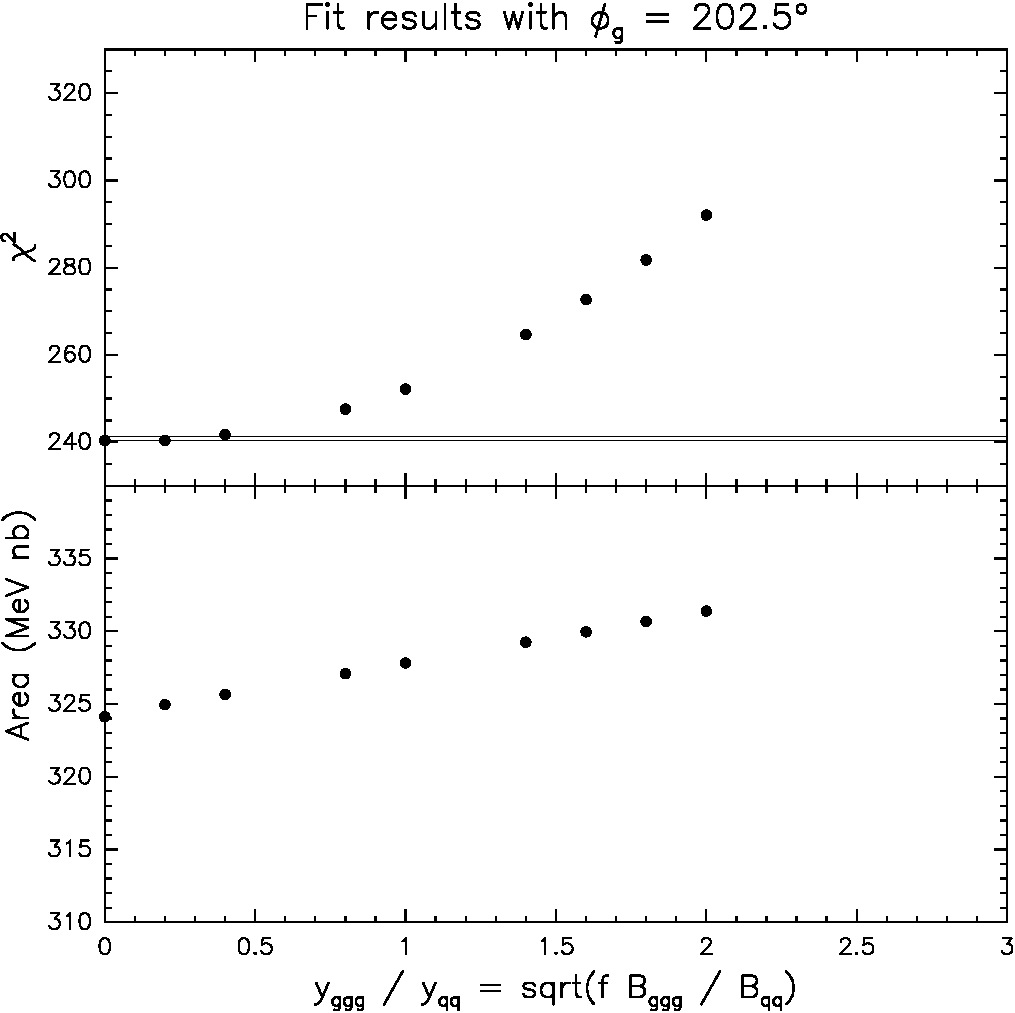
\includegraphics[width=\linewidth]{interference-j}

\vfill

\mbox{ }

\pagebreak

\mbox{ }

\vfill

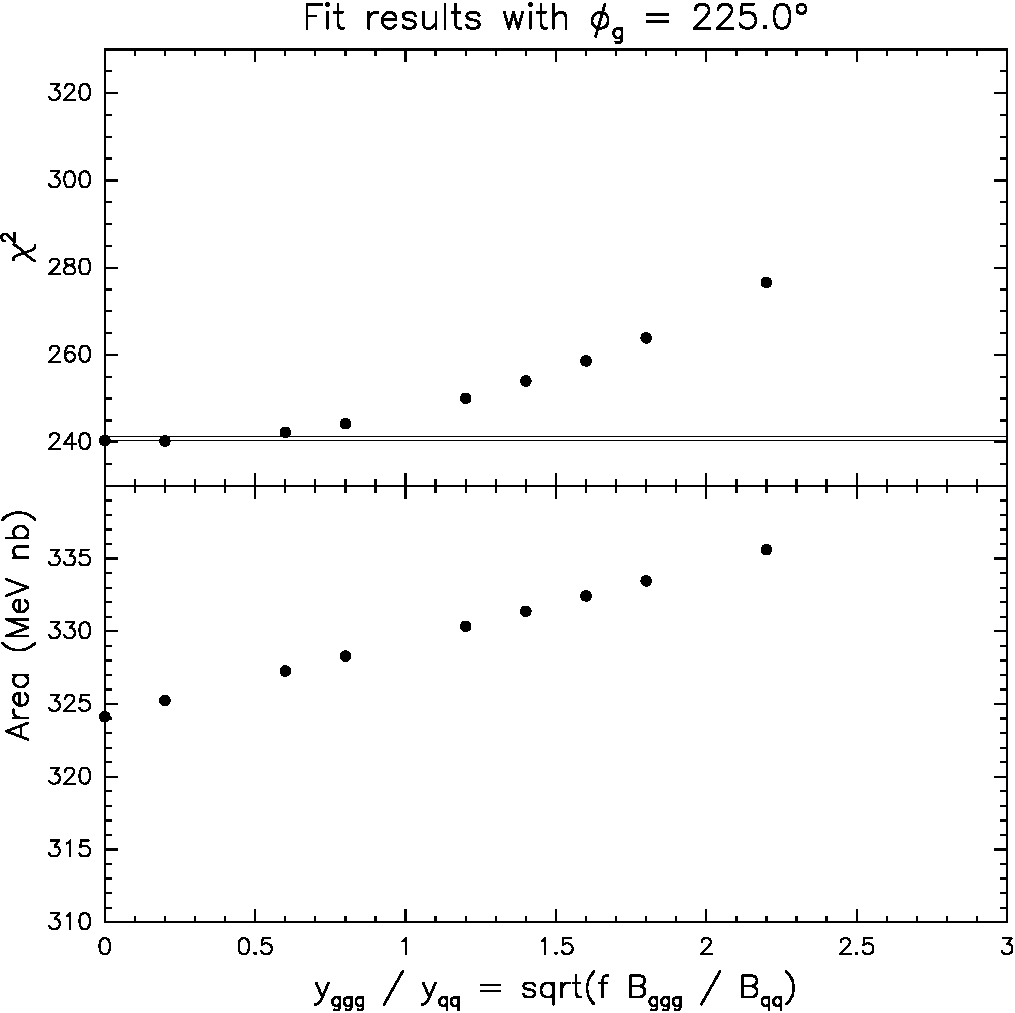
\includegraphics[width=\linewidth]{interference-k}

\vfill

\mbox{ }

\pagebreak

\mbox{ }

\vfill

\includegraphics[width=\linewidth]{interference-l}

\vfill

\mbox{ }

\pagebreak

\mbox{ }

\vfill

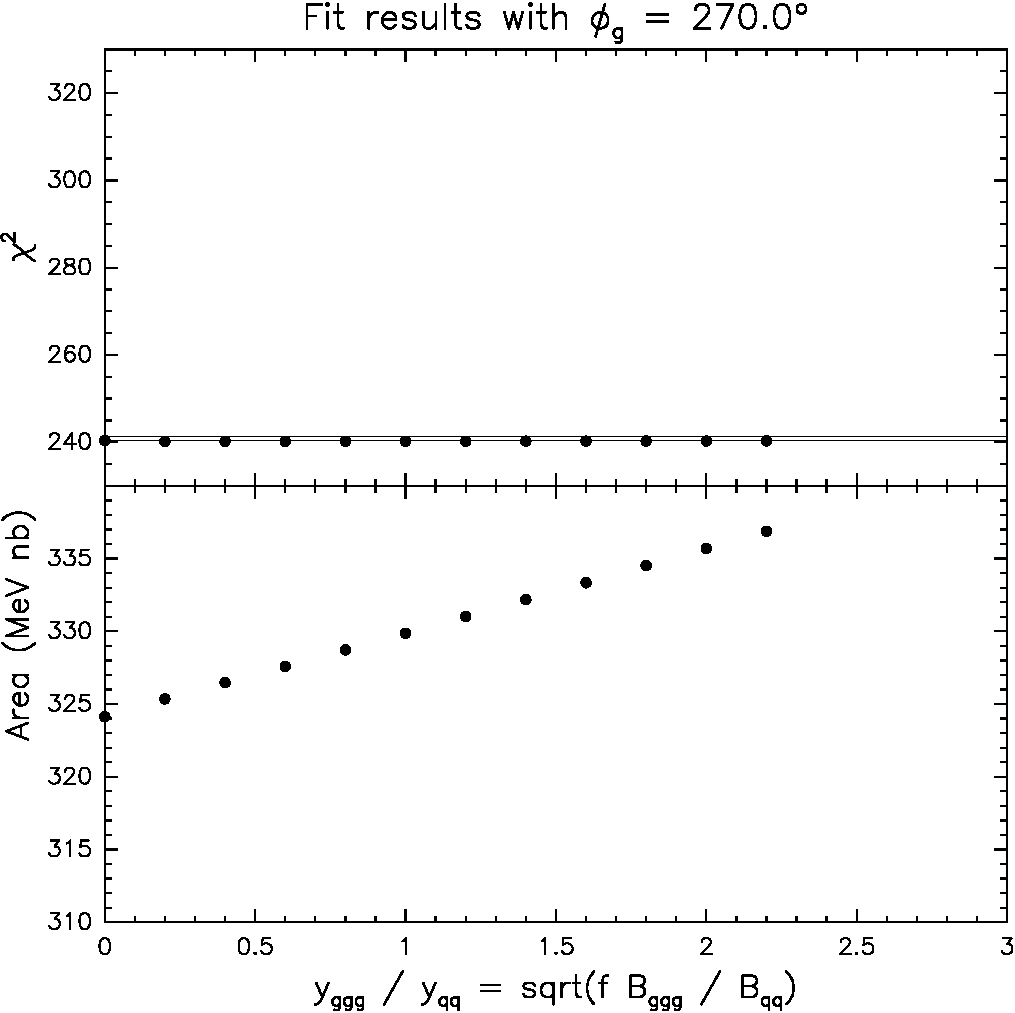
\includegraphics[width=\linewidth]{interference-m}

\vfill

\mbox{ }

\pagebreak

\mbox{ }

\vfill

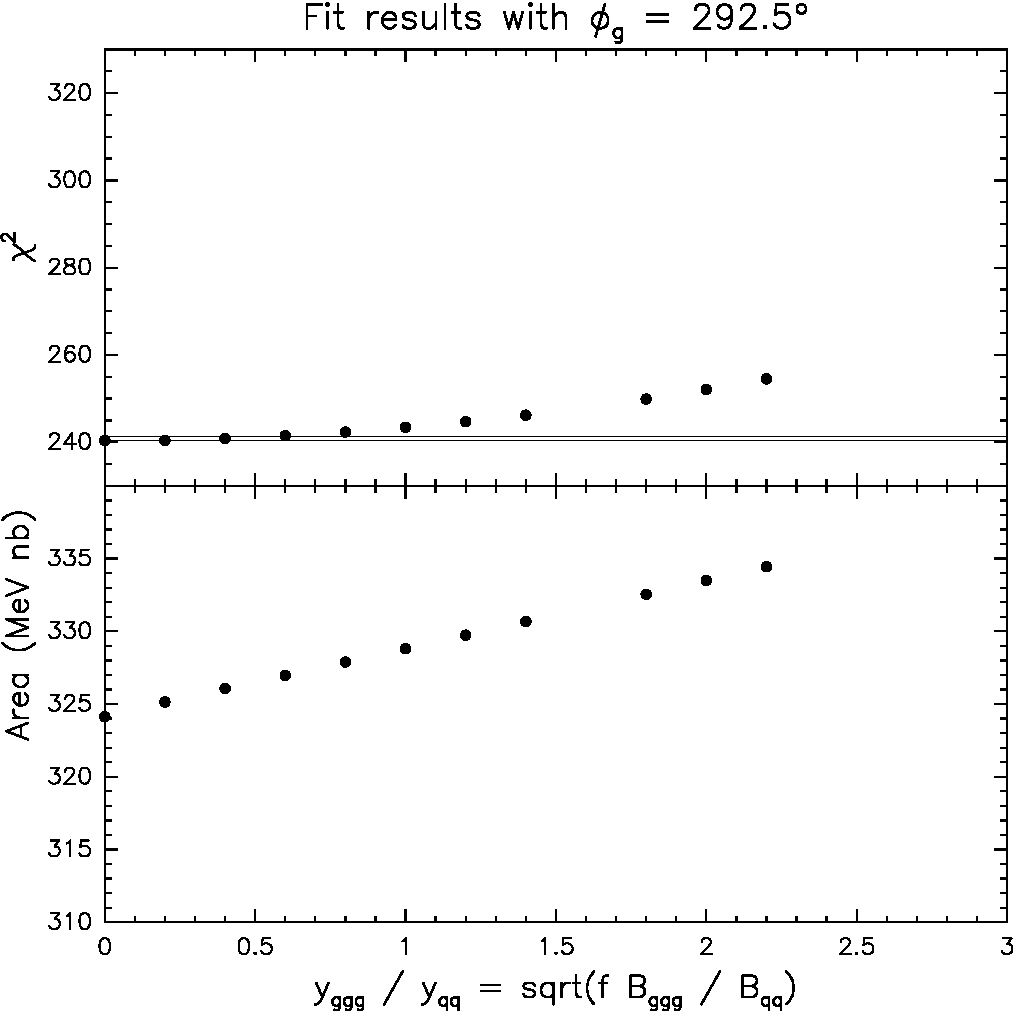
\includegraphics[width=\linewidth]{interference-n}

\vfill

\mbox{ }

\pagebreak

\mbox{ }

\vfill

\includegraphics[width=\linewidth]{interference-o}

\vfill

\mbox{ }

\pagebreak

\mbox{ }

\vfill

\includegraphics[width=\linewidth]{interference-p}

\vfill

\mbox{ }

\pagebreak

\section*{Other Forms of Interference}

\begin{center}
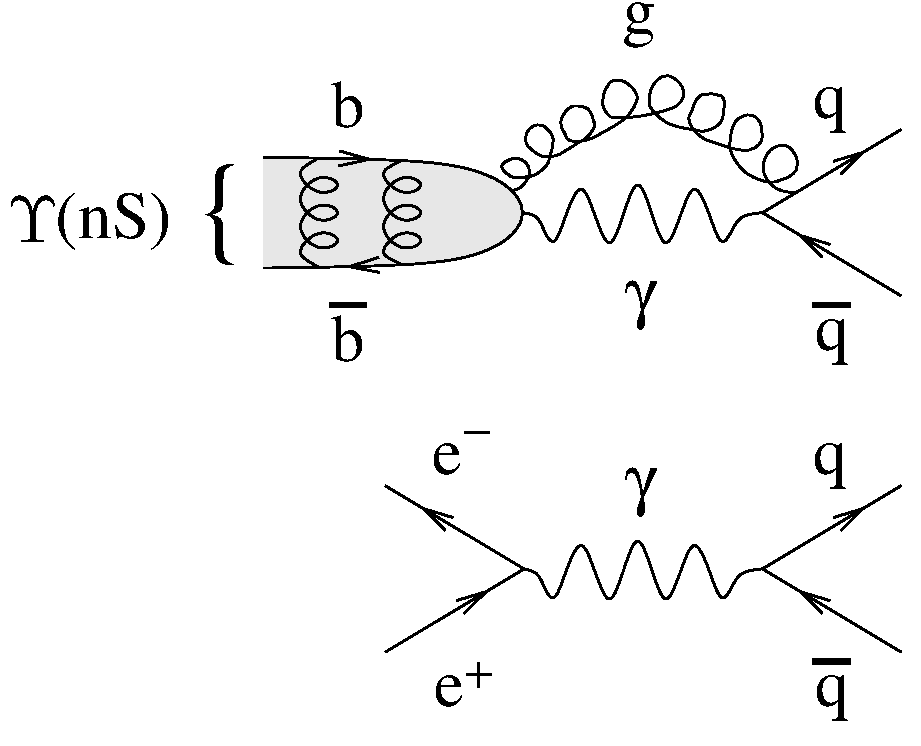
\includegraphics[width=0.5\linewidth]{interference-qqonly}
\end{center}

We have assumed that the $\sqrt{s} \ll M_\Upsilon$ phase difference
between continuum $q\bar{q}$ and $\Upsilon \to q\bar{q}$ is zero, as
it is for $\mu^+\mu^-$.  A gluon connecting $b\bar{b}$ with $q\bar{q}$
could spoil that.  However, the final state quarks are light (how
often are they $c\bar{c}$?), with $\sim$5 GeV of momentum, so
$\alpha_s$ is 0.2.  The top diagram is therefore of order 4\% on a
10\% decay mode.

\vfill

\begin{center}
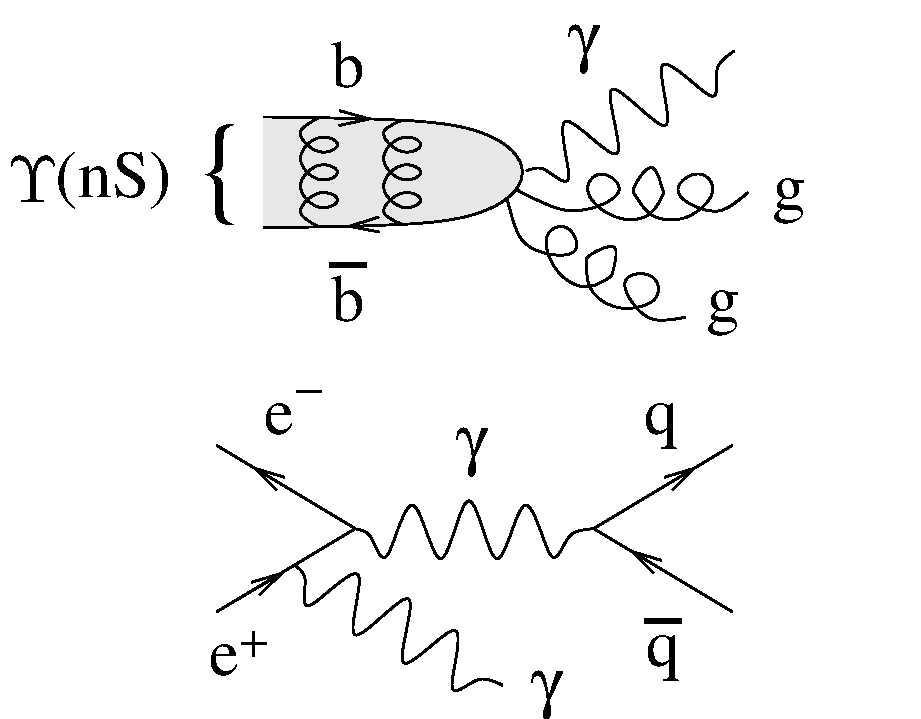
\includegraphics[width=0.5\linewidth]{interference-gggamma}
\end{center}

This is a very small effect because the $gg\gamma$ mode has a
branching fraction of some 3\%.

\vfill

\section*{Did I leave anything out?  Are my arguments wrong?}

\end{document}
